\chapter{ Maximização do coeficiente \dmc utilizando matriz \pdcca~e $DPDCCA$}\label{cap:paper_03}



\begin{flushright}
    ``Noel Meyerhof consulted the list he had prepared \\
    and chose which item was to be first. \\
    As usual, he relied mainly on intuition.''\\[10px]
    (Isaac Asimov)
    % Isaac Asimov - Jokester - 1956
    \end{flushright}

\begin{figure}[!htb]
	\centering
	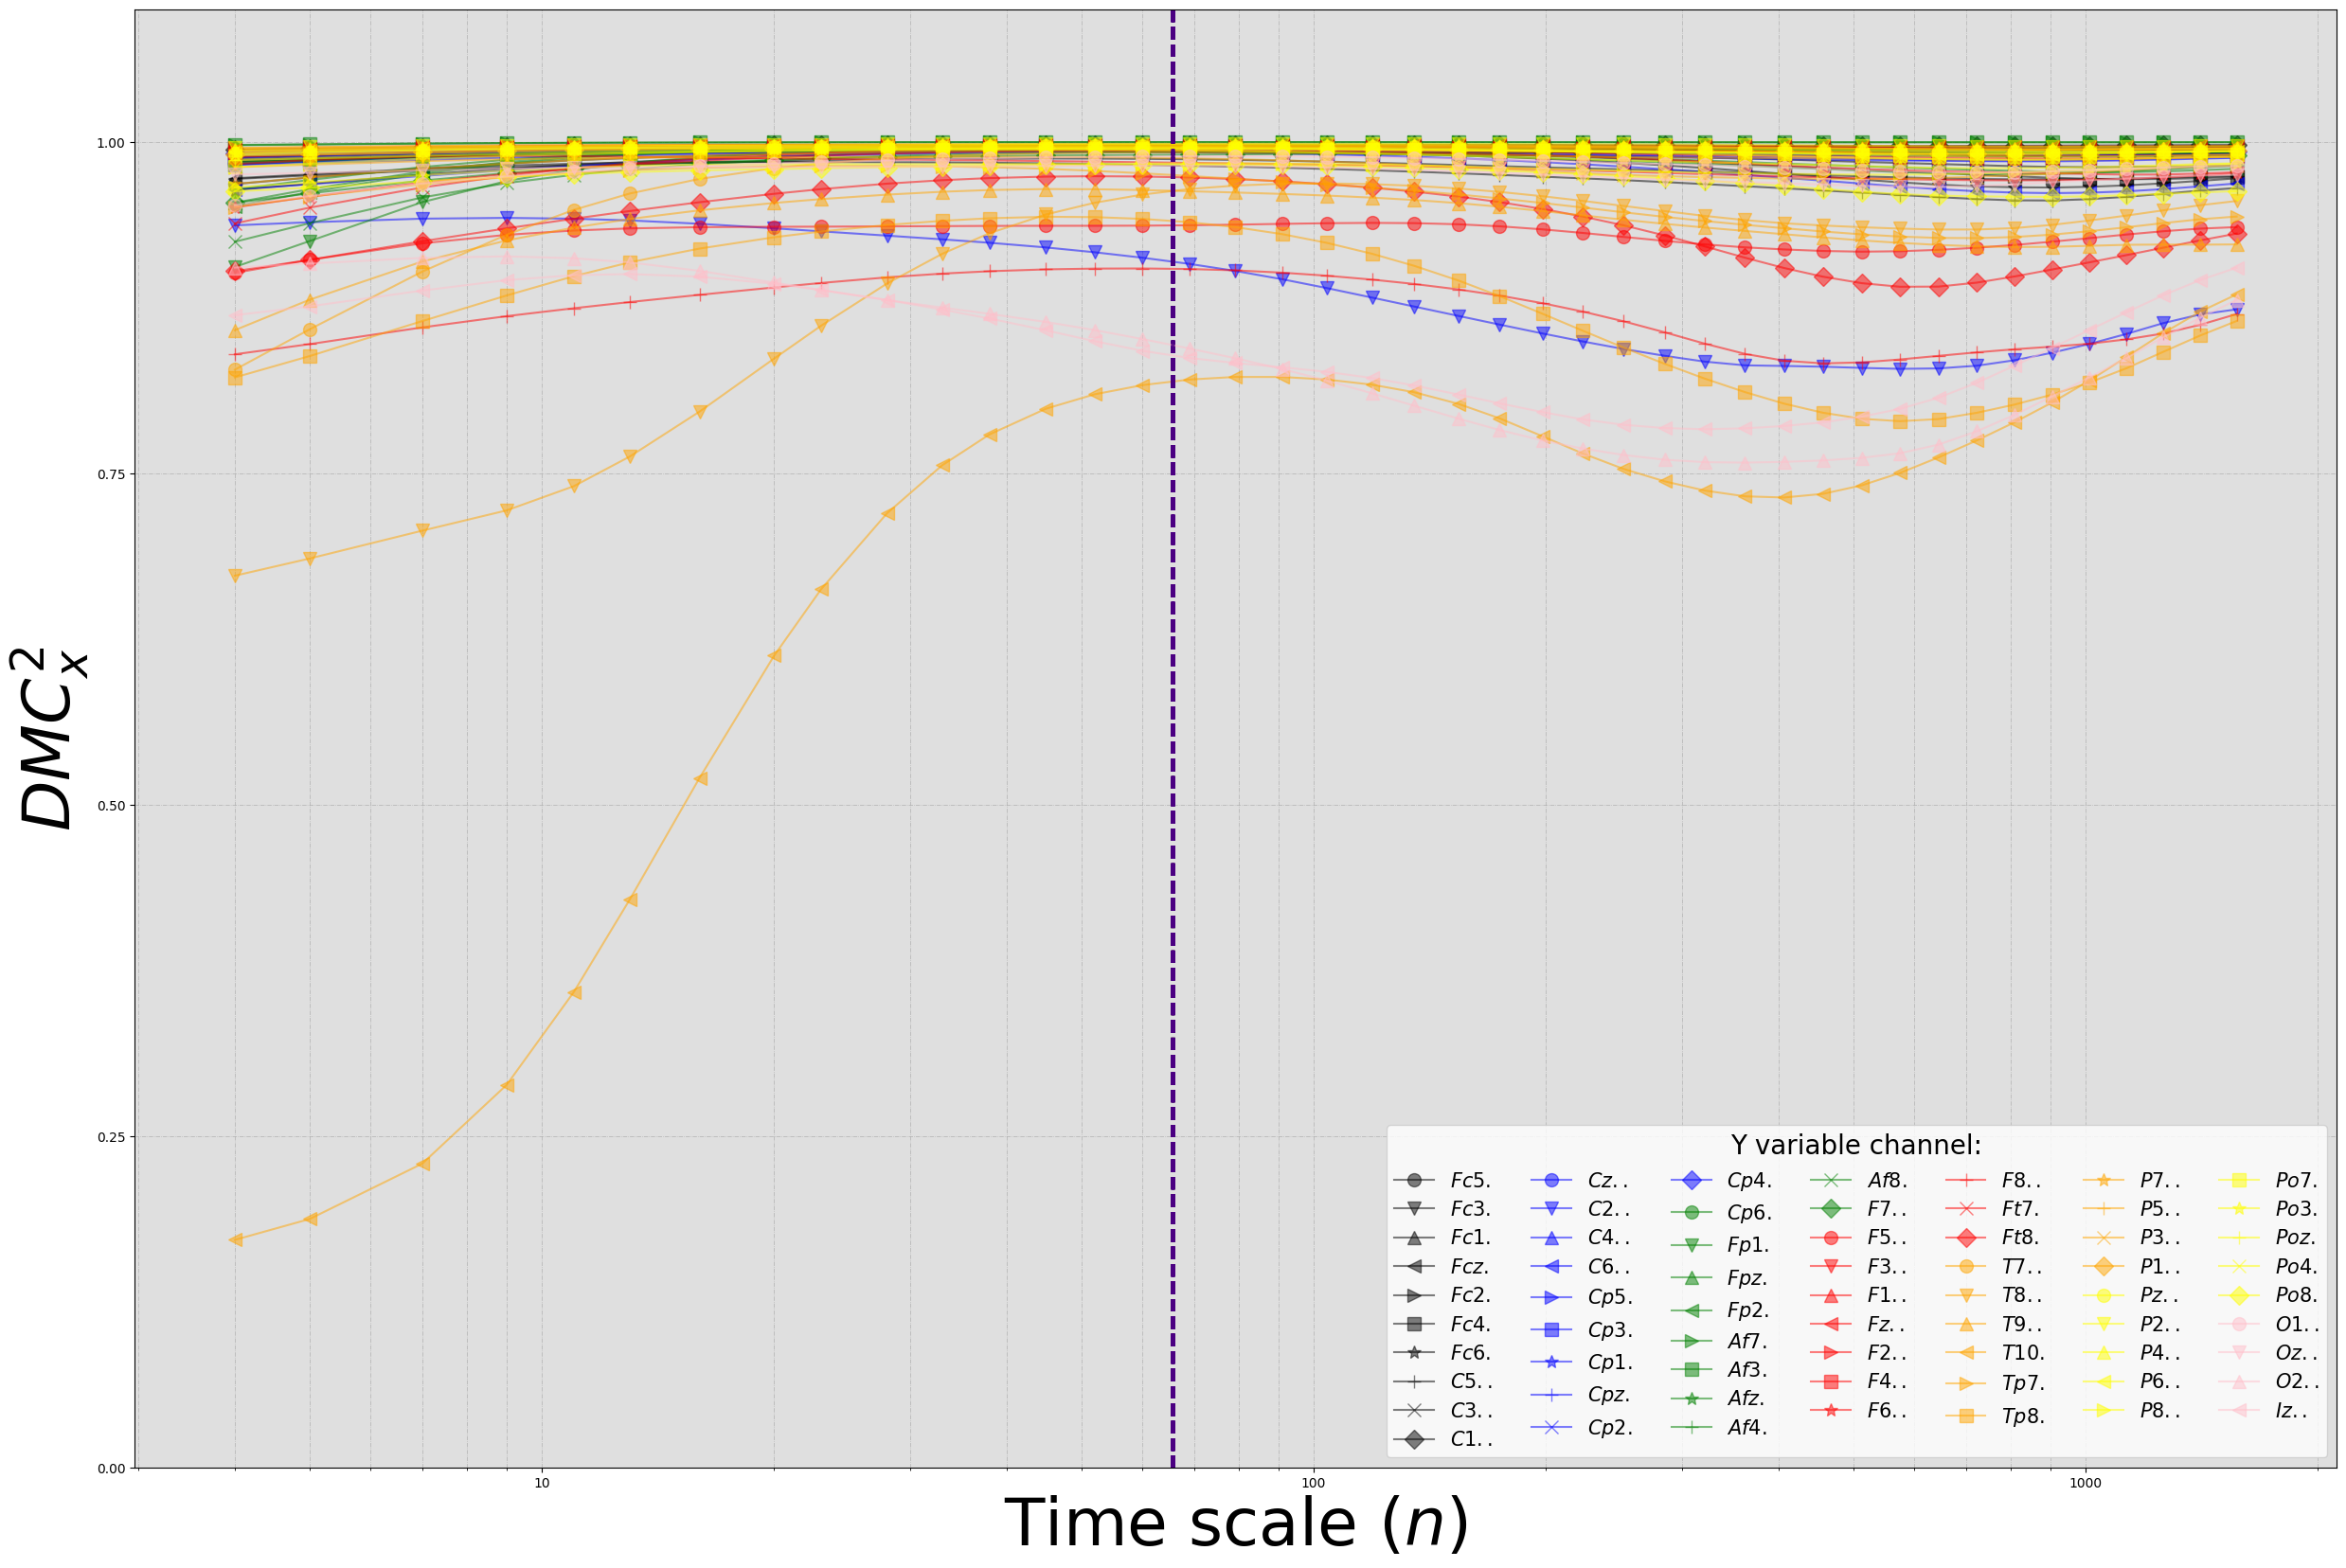
\includegraphics[width=.95\textwidth]{./Figures/art_03/dmc_all.png}
  \captionsetup{justification=centering}
  \caption{\dmc~de todo os canais do experimento[1:63] para cada canal como variável dependente.\\Fonte: Elaborada pelos autores}

	\label{fig:a03_dmc_total}
\end{figure}

Com a ferramenta desenvolvida e testada, volta-se para os dados utilizados nos artigos do Capítulo~\ref{cap:paper_01}, e no Anexo~\ref{an:a}. A matriz do \pdcca~para todos os $64$ canais é calculada em menos de $17min$. Isso se deve ao Algoritmo \emph{Detrended Saved}. Sem a aplicação deste, calculando o número de combinações necessárias para a montagem da matriz (Equação~\ref{eq:combinations_2x2}), levando em conta que, para cada \dcca~aplica-se duas vezes o cálculo do $DV$, chega-se ao valor de $2016 \times 2 = 4032$. Com o uso do algoritmo, apenas $64$ valores são calculados.

Com a matriz montada, o cálculo do \dmc, envolvendo todas as $64$ séries, com cada uma delas como variável dependente, para os $42$ valores de $n$, utilizados nos referidos artigos, é realizado em $0.7s$.

A Figura~\ref{fig:a03_dmc_total} apresenta esses resultados. Apontando para um sistema altamente correlacionado. Também encontramos um pico de correlação entre as escalas $n=60$ e $n=69$, confirmando o encontrado nos artigos.

A inversa de cada uma das $42$ matrizes do \pdcca~também foi calculada em menos de $1s$. O $DPDCCA$ foi implementado e calculado para todas as combinações de canais, para cada escala temporal, levando também menos de $1s$ na execução.

É evidente o aumento na quantidade de informações que se pode obter e tratar com as ferramentas computacionais desenvolvidas neste trabalho. É necessário desenvolver instrumentos para acessar essas informações.



 

\section{Metodologia}

Um experimento foi montado, investigando o quanto partindo da premissa:

\begin{itemize}
  \item Nem todos os canais contribuem igualmente para o \dmc~de uma série como variável dependente e todas as outras como dependente;

\end{itemize}

foram elaboradas a hipótese:

\begin{itemize}
  \item é possível selecionar um subconjunto pequeno de canais cujo \dmc~se aproxime do valor total.
\end{itemize}

Para testar a hipótese, foi escolhido o canal \emph{T8..}. Em um sistema tão correlacionado, um canal que, para $n=4$ afasta-se muito do conjunto mais correlacionado e, no pico de multi-correlação mostrado na Figura~\ref{fig:a03_dmc_total}, aproxima-se do citado conjunto, aparenta-se como um candidato interessante para as primeiras avaliações.

Optou-se pela escolha do \dmc de $1:8$ canais, representando $1/8$ do total de canais, para comparar com o valor do \dmc$1:64$. As escalas temporais $n=4$ e $n=69$ foram escolhidas.

Foram estabelecidos cinco modelos para escolher os 8 canais que mais contribuem para o \dmc~total:

\begin{itemize}
  \item Aleatório: como um artifício de controle.
  \item \pdcca : Os oito maiores valores do \pdcca de \emph{T8..} em relação À cada uma das outras variáveis.
  \item $|$\pdcca$|$ : Os oito maiores valores absolutos do \pdcca de \emph{T8..} em relação À cada uma das outras variáveis.
  \item $DPDCCA$ : Os oito maiores valores do $DPDCCA$ de \emph{T8..} em relação À cada uma das outras variáveis.
  \item $\Sigma DPDCCA$ : Um algoritmo baseado nas características do $DPDCCA$.  
\end{itemize}


\begin{algorithm} \caption{$\Sigma DPDCCA$} \label{alg:edpdcca}
  \begin{lstlisting}
  def maximize_dmc_dp(n, index, count, c_mat ):
    dmc_of = [index]
    for i in range(count):
        comp_array = np.full(64, fill_value = np.nan, dtype = float)
        for j in range(64):
            if j in dmc_of:
                pass
            else:
                for k in dmc_of:
                    temp = pddcca(j, k, n, c_mat)
                    if  np.isnan(comp_array[j]):
                        comp_array[j] = temp
                    else:
                        comp_array[j] += temp
        dmc_of.append(int(np.nanargmax(comp_array)))
    return np.array(dmc_of)

    \end{lstlisting}
\end{algorithm}

O critério de seleção $\Sigma DPDCCA$ aparece está apresentado, em código, no Algoritmo~\ref{alg:edpdcca}. O $DPDCCA$ tem características particulares. Analisando a Equação~\ref{eq:dpdcca} ve-se que, entre duas séries idênticas, obtêm-se o valor mais baixo possível $-1$, indicando que a informação daquela série não agrega valor ao todo.

Pelo critério do $\Sigma DPDCCA$, a escolha dos 8 canais acontece de forma sucessiva. O primeiro canal é escolhido pelo maior valor do $DPDCCA$ em relação ao canal \emph{T8}. Para os próximos $7$ canais, calcula-se o maior valor do $DPDCCA$ entre o canal candidato e o canal \emph{T8} somado com os valores de $DPDCCA$ entre o canal candidato e os canais escolhidos nas etapas anteriores.


\section{resultados}

A Tabela~\ref{tab:time_4} apresenta os resultados dos cinco métodos para $n=4$. O valor de referência é o valor do \dmc~de \emph{T8} com todos os outros canais. Os métodos aparecem na primeira coluna, Os canais selecionados na segunda, o valor do \dmc~de \emph{T8} em relação aos canais selecionados na terceira e o percentual do valor obtido em relação ao valor de referência na última coluna.

\begin{table}[h!]
    \centering
    \caption{Maximização do \dmc. $n=4,~ count=8$, referência$= 0.6726$} \label{tab:time_4}
    \begin{tabular}{c|c|c|c}
      \hline
      Critério & canais selecionados & valor & percentual \\
      \hline
      \hline
      \pdcca & T8 Fc6 C6 Cp6 F6 F8 Ft8 P4 P6 & 0.6330  & 94.1108\% \\
      $|$ \pdcca $|$ & T8 Fc6 C6 Cp6 F6 F8 Ft8 P4 P6  & 0.6330 & 94.1108\% \\
      $\Sigma DPDCCA$ & T8 Fc6 C6 Cp6 F2 F4 F6 F8 Ft8 & 0.6329 &  94.0908\% \\
      $DPDCCA$ & T8 C6 Cp6 Fp2 Afz F3 F4 Ft8 P6 & 0.5686 & 84.5341\% \\
      Random & T8 P6 P5 C1 F1 F4 Cp6 Fc1 F6 & 0.3138 & 46.6517\% \\
      
      \hline
    \end{tabular}
  \end{table}

  Os valores do \pdcca, do $|$ \pdcca $|$~ e do $\Sigma DPDCCA$ aproximam em tono de $94.1\%$, com o \pdcca, e o $|$ \pdcca $|$~escolhendo os mesmos canais e performando levemente acima do $\Sigma DPDCCA$, que escolheu os canais \emph{F2} e \emph{F8} em vez dos canais \emph{P4} e \emph{P6}. O desempenho do critério $DPDCCA$ fica abaixo dos já citados.

  \begin{table}[h!]
    \centering
    \caption{Maximização do \dmc. $n=69,~ count=8$, referência$=0.9643 $} \label{tab:time_69}
    \begin{tabular}{c|c|c|c}
      \hline
      Critério & canais selecionados & valor & percentual \\
      \hline
      \hline
      \pdcca & T8 Fc4 Fc6 C4 C6 Cp6 F6 Ft8 Tp8 & 0.9581  & 99.3548\% \\
      $|$ \pdcca $|$ & T8 Fc4 Fc6 C4 C6 Cp6 F6 Ft8 Tp8  & 0.9581 & 99.3548\% \\
      $\Sigma DPDCCA$ & T8 Fc6 C6 Cp6 Ft8 T10 Tp8 P6 P8 & 0.9597 &  99.5189\% \\
      $DPDCCA$ & T8 C6 Cp6 Ft8 T7 T10 Tp7 Tp8 P8 & 0.9572 & 99.2568\% \\
      Random & T8 Fp1 Po7 F7 P6 Cp3 C3 Po4 P2 & 0.8083 & 83.8165\% \\
      \hline
    \end{tabular}
  \end{table}

  Na tabela~\ref{tab:time_69} ve-se resultados semelhantes. Nesta escala temporal com maior multi-correlação, aparece o $\Sigma DPDCCA$ um pouco acima dos outros e com o critério $DPDCCA$ mais próximos dos demais. Diferenças entre os canais escolhidos em uma escala temporal para a outra também foram registrados.

  A semelhança entre os critérios \pdcca~e $|$ \pdcca $|$~ se deve à característica do sistema de além de ser fortemente muli-correlacionado, também é positivamente multi-correlacionado. Desconsiderando o \pdcca~de um canal com ele mesmo, os valores de \pdcca~variam de $0.9995$ até o mínimo de $-0.2281$. Não existem anti-correlações significativas em nenhuma das escalas temporais calculadas. 

  \section{Conclusão}

Os critérios $|$ \pdcca $|$~e $\Sigma DPDCCA$~apresentaram bons resultados na maximização do coeficiente \dmc em relação ao total. É recomendado a repetição do experimento em mais escalas temporais e com outros canais como variável dependente.

Os critérios de aproximação também podem ser entendidos como critérios de semelhança entre séries. Se bem entendidos e validados por extensões desta pesquisa.

A ideia de maximizar o coeficiente apresenta similaridades com o processo de seleção de atributos em um algoritmo de aprendizado de máquina. Os resultados preliminares podem ser entendidos como um indício de que o desempenho destes critérios para a seleção de atributos devem ser verificados.


 

